\pagebreak
\hypertarget{Errores}{\section{Posibles errores}}

    \begin{itemize}
        \item Problemas con la conexión o el sistema

        Si al momento de acceder a alguna  pantalla, aparece el siguiente mensaje:
                %Imagen MSG7 Y MSG25

        \begin{figure}[!hbtp]
            \centering
            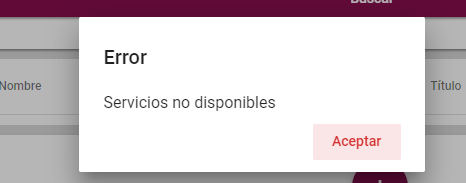
\includegraphics[width=0.4\linewidth]{images/SP6/MSGSN.png}
            \caption{Servicios no disponibles}
            \label{SND}

        \end{figure}
        
        Significa que existió un error de conexión o del sistema. Al dar clic en en botón ''Aceptar'', el sistema lo redireccionará a la pantalla anterior. Deberá esperar a que la página este disponible para  intentar acceder nuevamente.

        \item Campos vacíos al momento de ingresar el registro. 

        Si usted deja en blanco algún campo o campos del formulario, y posteriormente dio clic en \IUbutton{Finalizar}, el sistema mostrará el siguiente mensaje debajo del campo o campos :
                
        \begin{figure}[!hbtp]
            \centering
            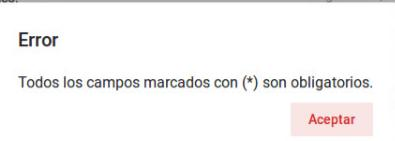
\includegraphics[width=0.4\linewidth]{images/SP6/Vacios.jpeg}
            \caption{Campos vacíos}
       \end{figure}

       Regresara al formulario, en donde usted deberá llenar el o los campos que dejo vacíos.
       
         \pagebreak
       \item Los campos ingresados no son válidos
       
       Si al momento de dar clic en \IUbutton{Finalizar} aparece el siguiente mensaje:
        \begin{figure}[!hbtp]
            \centering
            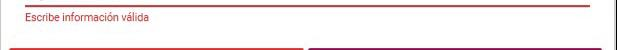
\includegraphics[width=0.4\linewidth]{images/SP6/Invalida.jpeg}
            \caption{Campos incorrectos}
        \end{figure}

        Significa que la composición de los datos ingresados en el formulario no es la correcta. 
    
    \end{itemize}
    